\documentclass[12pt, letterpaper]{standalone}

\usepackage{titling}
\usepackage{standalone}
\usepackage{fontenc}


\usepackage[x11names]{xcolor}
\definecolor{SaddleBrown}{rgb}{0.55, 0.27, 0.07}
\definecolor{IndianRed}{rgb}{0.80, 0.36, 0.36}
\definecolor{Firebrick}{rgb}{0.70, 0.13, 0.13}
\definecolor{DarkBlue}{rgb}{0, 0, 0.55}
\definecolor{Goldenrod}{rgb}{0.85, 0.65, 0.13}
\definecolor{Peru}{rgb}{0.85, 0.65, 0.13}




\usepackage{hyperref}
\hypersetup{
    colorlinks=true,
    linkcolor=DarkBlue,
    urlcolor=blue,
    linktoc=all
}
\setcounter{tocdepth}{1}


\usepackage{mathtools}
\usepackage{amsmath}
\usepackage{tikz}
\usepackage{verbatim}
\usetikzlibrary{calc}

% put color to \boxed math command
\newcommand*{\boxcolor}{Peru}
\makeatletter
\renewcommand{\boxed}[1]{\textcolor{\boxcolor}{%
\tikz[baseline={([yshift=-1ex]current bounding box.center)}] \node [rectangle, minimum width=1ex,rounded corners,draw] {\normalcolor\m@th$\displaystyle#1$};}}
\makeatother


\usepackage{listings}

\definecolor{codegreen}{rgb}{0,0.6,0}
\definecolor{codegray}{rgb}{0.5,0.5,0.5}
\definecolor{codepurple}{rgb}{0.58,0,0.82}
\definecolor{backcolour}{rgb}{0.95,0.95,0.92}

\lstdefinestyle{mystyle}{
    backgroundcolor=\color{backcolour},
    commentstyle=\color{codegreen},
    keywordstyle=\color{magenta},
    numberstyle=\tiny\color{codegray},
    stringstyle=\color{codepurple},
    basicstyle=\ttfamily\footnotesize,
    breakatwhitespace=false,
    breaklines=true,
    captionpos=b,
    keepspaces=true,
    numbers=left,
    numbersep=5pt,
    showspaces=false,
    showstringspaces=false,
    showtabs=false,
    tabsize=2
}

\lstset{style=mystyle}


\usetikzlibrary{positioning}
\usetikzlibrary{petri} % LATEX and plain TEX
\usetikzlibrary[petri] % ConTEXt
\usepackage{pgfplots}
\pgfplotsset{compat=1.13}


\usepackage{framed}
\usepackage{quoting}

\colorlet{shadecolor}{LightSteelBlue1}
\usepackage{lipsum}
\newenvironment{shadedquotation}
 {\begin{shaded*}
  \quoting[leftmargin=5pt, rightmargin=5pt, vskip=0pt]
 }
 {\endquoting
 \end{shaded*}
}


\usepackage{lipsum} % for dummy text
\usepackage{enumitem}
\setlist{nosep} % or \setlist{noitemsep} to leave space around whole list

\pagestyle{plain}

\usepackage{ctex}
\usepackage{xeCJK}
\xeCJKsetup{CJKmath=true}


\begin{document}

\pagestyle{empty}


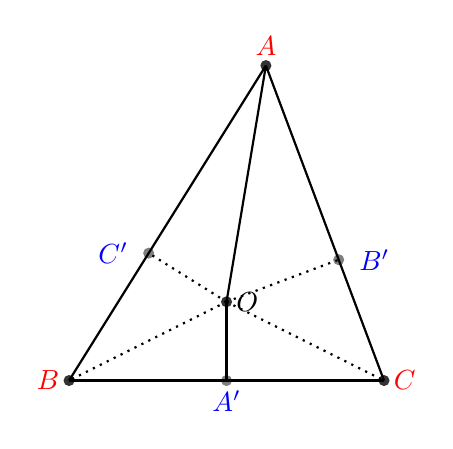
\begin{tikzpicture}
\coordinate [label=above:\textcolor{red}{$A$}] (A) at (0.5,4);
\coordinate [label=left:\textcolor{red}{$B$}] (B) at (-2,0);
\coordinate [label=right:\textcolor{red}{$C$}] (C) at (2,0);
\coordinate [label=right:\textcolor{black}{$O$}] (O) at (0,1);

\coordinate [label=below:\textcolor{blue}{$A'$}] (A_1) at (0,0);

\draw[black, thick] (A) -- (B) node(A_B_line)[] {};
\draw[black, thick] (B) -- (C);
\draw[black, thick] (C) -- (A);
\draw[black, thick] (O) -- (A_1);
\draw[black, thick, dotted] (O) -- (B);
\draw[black, thick, dotted] (O) -- (C);
\draw[black, thick] (O) -- (A);


\draw[black, thick, dotted] (O) -- ($(A)!(O)!(B)$) node(C_1)[label=left:\textcolor{blue}{$C'$}] {};
\draw[black, thick, dotted] (O) -- ($(A)!(O)!(C)$) node(B_1)[label=right:\textcolor{blue}{$B'$}] {};

\foreach \point in {A,B,C, O}
\fill [black,opacity=.8] (\point) circle (2pt);

\foreach \point in {A_1, B_1, C_1}
\fill [black,opacity=.5] (\point) circle (2pt);


\end{tikzpicture}

\end{document}
